\documentclass{article}
\usepackage[utf8]{inputenc}
\usepackage[serbian]{babel} 
\usepackage{listings}
\usepackage{graphicx}
\usepackage{tikz}
\usepackage{color, colortbl}
\definecolor{Gray}{gray}{0.9}
\usepackage[table,xcdraw]{xcolor}
\usepackage{hyperref}
\hypersetup{
colorlinks,
linkcolor=blue,
urlcolor=blue
}
\setlength{\textheight}{600pt}
\setlength{\textwidth}{140mm}
\setlength{\topmargin}{5pt}
\setlength{\evensidemargin}{53pt}
\setlength{\oddsidemargin}{10mm}

\title{%
  Spam detection using a multi-layer perceptron \vspace{0.4cm} \\ 
  \large Projekat u okviru kursa Računarska inteligencija \\
  Matematički fakultet\\ Univerzitet u Beogradu \vspace*{0.5cm}}
  
\author{Đorđe Milošević \\
\href{mailto:mi17105@alas.matf.bg.ac.rs}{mi19221@alas.matf.bg.ac.rs} \\
}

\date{\vspace*{1cm}April 2023}

\begin{document}

\maketitle

\newpage

\renewcommand*\contentsname{Sadržaj}
\tableofcontents
\newpage

\section{Opis problema}
Data je \href{https://github.com/Djolka/Spam-detection-using-a-multi-layer-perceptron/blob/main/emails.csv}{baza} email poruka koja sadrzi 2 kolone. Prva kolona pod nazivom \textit{text} sadrzi datu poruku koju je potrebno obraditi, dok druga kolona pod nazivom \textit{spam} sadrzi vrednosti 1, ukoliko je email poruka spam, ili 0, ukoliko poruka nije spam.
Cilj je napraviti model neuronske mreze koji ce pomocu vise slojeva efektivno da odredi da li je email poruka spam ili ne.

\section{Implementacija}
Podaci ce prvo biti pretprocesirani kako bi bili u pogodnom obliku za dalji rad. Nakon toga je potrebno obraditi dati sadrzaj poruka kako bi njihov oblik bio pogodan za rad sa neuronskim mrezama. Za to cemo koristiti TF-IDF matrice. Potrebno je izdvojiti sve reci koje se javljaju u email porukama i one ce ciniti kolone nase TF-IDF matrice. Zatim ce podaci biti podeljeni na 2 skupa, \textit{train} i \textit{test}, kako bismo mogli da istreniramo nas model na jednom skupu i pravilno da testiramo na drugom. Nakon toga cemo napraviti nasu viseslojnu neuronsku mrezu. Za kraj cemo videti ocenu kvaliteta naseg modela pomocu matrice konfuzije, ocene preciznosti itd.  

\subsection{Obrada ulaznih podataka}
Ulazni podaci se nakon ucitavanja pretprocesiraju. Prvo se uklanjaju duplikati zarad efikasnosti u daljem toku rada, a zatim se proverava da li postoje neke \textit{null} vrednosti podataka i uklanjaju se ako takve postoje.\\
Podatke je zatim potrebno podeliti u 2 grupe. Prva grupa ce sadrzati podatke koji se nalaze u koloni \textit{text} i oznacavacemo ih sa \textit{X}, a druga grupa ce sadrzati podatke koji se nalaze u koloni \textit{spam} i oznacavacemo ih sa \textit{y}. Ova podela nam dalje sluzi za treniranje podataka, kao i za ocenu samog modela.\\

\subsection{Kreiranje CountVectorizer matrice}
Za kreiranje count vectorizer matrice koristicemo CountVectorizer iz biblioteke sklearn
\\

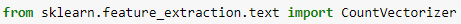
\includegraphics{countvectorizer.png}\\
\\
CountVectorizer se koristi sa ciljem da kolekciju tekstualnih dokumenata (u ovom slucaju mail-ovi) pretvori u vektor tokena gde za svaki token imamo koliko se puta ponavlja u svakom dokumentu (mail-u).
Iako je count vectorizer matrica solidna, TF-IDF matrica moze bolje da da znacaj odredjenim recima, i tako da nam da znacajniju i efikasniju matricu. Ona uzima u obzir ne samo broj ponavljanja reci u nekom dokumentu, vec i koliko je znacajna ta rec u nekom skupu dokumenata. Ovo se radi tako sto se "kazne" reci koje se cesto javljaju u dokumentima, cime se smanjuje njihov znacaj.

\newpage
\subsection{Kreiranje TF-IDF matrice}
Za kreiranje tf-idf matrice koristicemo \textit{TfidfVectorizer} iz biblioteke \textit{sklearn}\\

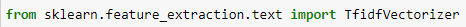
\includegraphics{tfidfInclude.png}\\
TF oznacava \textit{term frequency}, odnosno koliko puta se data rec javlja u jednom dokumentu u odnosu na ukupan broj reci datog dokumenta. Formula za izracunavanje TF vrednosti za rec \textit{t} u dokumentu \textit{d} je:\\

$$TF(t,d) = \frac{t}{d}$$\\
gde je t broj ponavljanja reci t u datom mail-u, a d je ukupan broj reci u mail-u.\\ 
IDF oznacava \textit{Inverse document frequency} odnosno \textit{inverznu frekvenciju dokumenta}.
IDF vrednost se odnosi na skup dokumenata (u ovom slucaju skup mail-ova). IDF nam sluzi da smanji znacaj reci koje se cesto javljaju, a poveca znacaj recima koje su retke. Formula za izracunavanje IDF vrednosti za rec t, u dokumentu d, koji pripada skupu dokumenata D je:

$$ IDF(t,d,D) = \log\frac{|D|}{|\{d\in D, t \in d\}|} $$\\
Na kraju za dobijanje TF-IDF vrednosti potrebno je da pomnozimo dve prethodno dobijene vrednosti:
$$TFIDF(t,d,D) = TF(t,d) * IDF(t,D)$$

\subsection{Word2Vec}
Word2Vec je tehnika pomocu koje se obradjuje prirodan jezik. Pomocu neuronske mreze uci o vezama izmedju odredjenih reci iz nekog skupa teksta. Ovaj model moze da pronadje sinonime reci, ili da dopuni parcijalno uredjene recenice. Svaka rec je predstavljena pomocu odredjene liste brojeva (vektor), koji se kao takav, moze upotrebiti moze ukazati na odredjene semanticke slicnosti izmedju reci predstavljenih tim vektorima. Ulaz u Word2Vec je skup tekstova, a izlaz je skup vektora koji predstavljaju te tekstove.\\
Postoje dve vrste treniranja reci: 
\begin{itemize}
    \item Koriscenje konteksta za predvidjanje ciljane reci (CBOW)
    \item Koriscenje reci za predvidjanje ciljanog konteksta (skip-gram)
\end{itemize}
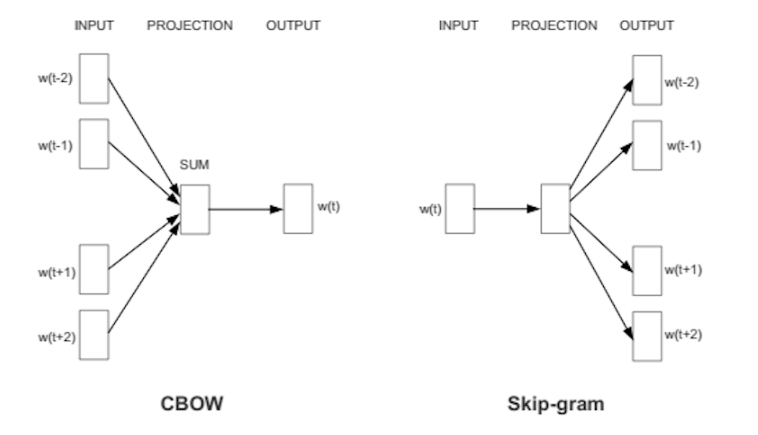
\includegraphics[scale=0.7]{word2vecpic.png}

Za nas model, u funkciji \textit{gensim.models.Word2Vec() } podesicemo paramtere \textit{window} i \textit{min\textunderscore count} kako bi nas model radio sto preciznije. Podesavanjem window parametra, primeceno je da za vrednosti od par stotina (od 100 do 700), i min\textunderscore count-a od oko 5 (ignorise sve reci koje imaju TF manji od ovog) dobijamo efikasan model koji nam daje preciznost od ~0.911.


\subsection{Train-test split}
Da bismo mogli da upotrebimo podatke tako da nas model moze na najbolji nacin da uci nad njima, moramo ih podeliti na \textit{train} i na \textit{test} skupove. Nad \textit{train} skupom cemo da istreniramo nas model, nakon cega ce model to steceno znanje da iskoristi u evaluaciji test podataka.\\


\subsection{Viseslojna neuronska mreza}
Za implementaciju viseslojne neuronske mreze koristi se \textit{tensorflow.keras} biblioteka: \\

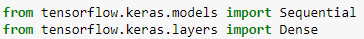
\includegraphics{tensorflow_keras.png}\\
\\
Mrezu cemo modelovati na trening podacima. U ulaznom sloju input\textunderscore dim ce biti X\textunderscore train.shape[1]. Posto nas problem predstavlja binarnu klasifikaciju u izlaznom sloju imamo samo jedan cvor, koji sadrzi vrednost [0,1]. Ako je vrednost iznad 0.5, mail je spam, a u suprotnom nije spam. Nakon definisanja nase mreze izvrsavamo kompiliranje naseg modela, gde optimizer postavljamo na \textit{adam}, loss na \textit{binary\textunderscore crossentropy} (jer je nas problem binaran), a za metrics koristimo \textit{accuracy}. Zatim fit-ujemo nas model na trening podacima, X\textunderscore train, i y\textunderscore train. Batch\textunderscore size , epochs i validation\textunderscore split ce biti podesavani.


\newpage
\subsection{Ocena modela}
Metode za ocenu modela cemo ukljuciti iz sklearn.metrics biblioteke:\\
\\
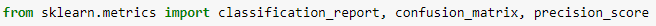
\includegraphics{metrics.png}\\
\\
Koristicemo \textit{classification\textunderscore report}, \textit{confusion\textunderscore matrix} kao i \textit{precision\textunderscore score}. \\
\textbf{Classification\textunderscore report} nam daje raznorazne metrike kao sto su recall, f1 score, accuracy...
\textbf{Confusion\textunderscore matrix:}\\
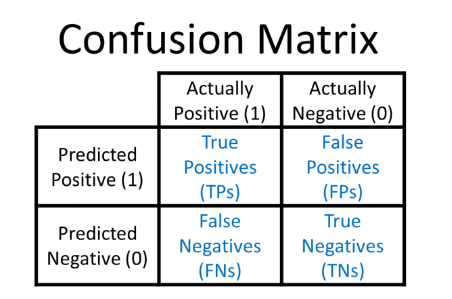
\includegraphics{confusion_matrix.png}\\
\\
\textbf{Precision\textunderscore score} se racuna pomocu formule:\\
$$\frac{TP}{(TP + FP)}$$ \\
Ove ocene ce nam pomoci u odlucivanju efikasnosti nase mreze i potencijalnoj optimizaciji iste.


 \newpage
\section{Rezultati modela}
Za aktivacionu funkciju ulaznog sloja cemo koristiti \textit{Relu} aktivacionu funkciju, a za aktivacionu funkciju izlaznog sloja cemo uvek koristiti \textit{sigmoidnu} funkciju: \\
\\
\\
 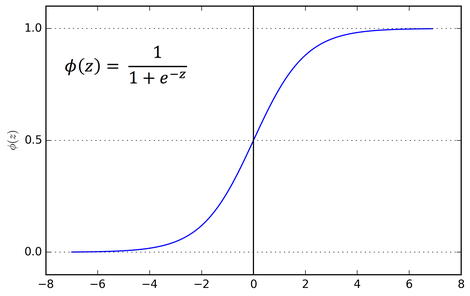
\includegraphics{sigmoid.png}\\
\\
Sigmoidna funkcija mapira ulazne vrednosti u interval [0,1] sto je pogodno za binarnu klasifikaciju koju koristimo.\\
\\
\textbf{Plave linije na plotovima ce oznacavati trening skup, dok ce narandzaste oznacavati validacioni skup.}\\
\\
\textbf{Pocetni model} ce sadrzati 2 sloja, ulazni i izlazni. \\
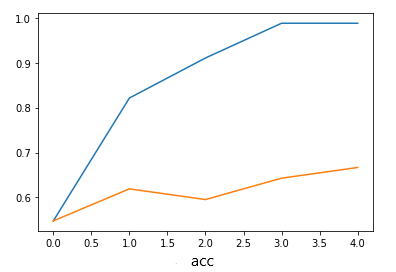
\includegraphics[scale=0.8]{acc.png}
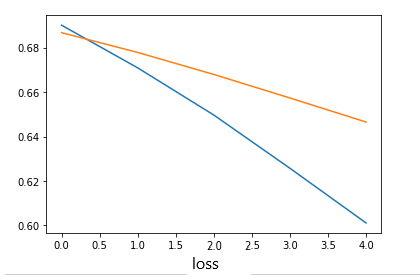
\includegraphics[scale=0.8]{loss.png}\\
\\
Levi plot predstavlja \textit{accuracy} kroz epohe, dok desni predstavlja \textit{loss}.\\
\\
U ovom modelu trening skup dolazi do tacnosti od 0.9881 dok validacioni skup dolazi do tacnosti od 0.7381.
Uz to vidimo da je loss na validacionom skupu veci nego na trening skupu, sto nam sve ukupno govori da je doslo do preprilagodjavanja podataka. Pokusacemo da poboljsamo nas model pomocu regularizacije iz biblioteke tensorflow:\\
\\
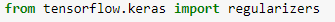
\includegraphics{regularizers.png}\\
\\
Regularizacija predstavlja razne tehnike koje smanjuju kompleksnost modela tokom treninga, sto sprecava preprilagodjavanje. Koristicemo L1 regularizaciju.\\
Nakon regularizacije primecujemo da nam je tacnost na validacionom skupu veca - 0.8810, dok je loss ostao slican kao i pre regularizacije. Vidimo da ovaj model jos moze da se optimizuje i sledeci korak nam je dodavanje skrivenih slojeva.\\
\\
\textbf{Poboljsani model} (dodavanje skrivenih slojeva)\\ 
U ovom modelu cemo dodati jedan skriveni sloj koji ce sadrzati 32 cvora, a za aktivacionu funkciju cemo koristiti \textit{relu} aktivacionu funkciju. Takodje cemo povecati i broj epoha na 10, sto znaci da ce nasi trening podaci proci veci broj kroz mrezu i time poboljsati parametre same mreze.\\ \\ \\ \\
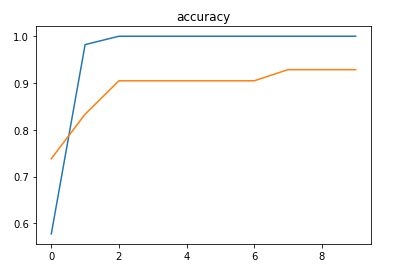
\includegraphics[scale=0.8]{acc2.png}
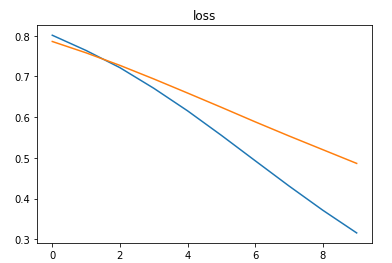
\includegraphics[scale=0.8]{loss2.png}\\
\\
Nakon dodavanja samo jednog skrivenog sloja vidimo poboljsanje modela, gde je sada tacnost 0.928 na validacionom skupu, sa loss-om od 0.4863.
Pokusacemo da ga poboljsavamo dodavanjem skrivenih slojeva. Novi skriveni sloj ce da sadrzi 64 cvora i takodje ce da koristi \textit{relu} aktivacionu funkciju. Povecacemo i broj epoha na 40 kako bi parametri sto bolje bili podeseni.\\
\\
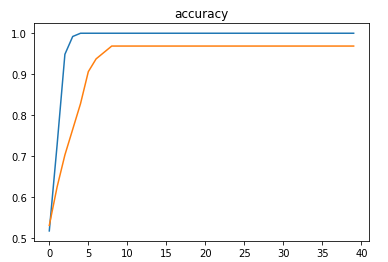
\includegraphics[scale=0.8]{acc3.png}
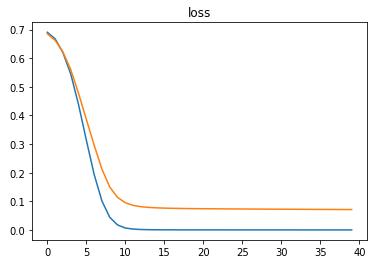
\includegraphics[scale=0.8]{loss3.png}\\
\\
Nakon dodavanja i drugog skrivenog sloja tacnost na validacionom skupu je sada 0.9688, a loss je 0.0712, sto predstavlja poboljsanje u odnosu na jedan skriveni sloj.\\
Dodavanjem jos skrivenih slojeva primecuje se da mreza ne napreduje sto znaci da su 2 sloja optimalna. Na test skupu dobijamo tacnost od 0.9854 sa lossom od 0.04.\\
Ostale ocene su date u sledecoj tabeli:\\ 
\\
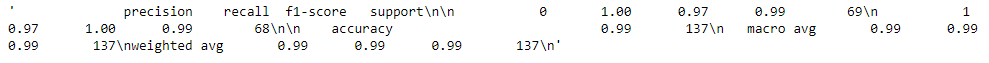
\includegraphics[scale=0.65]{class_report.png}\\
\\
Kao i matrica konfuzije:\\ 
\\
$$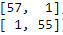
\includegraphics[scale=2]{conf_matrix.png}\\$$
\\
\section{Zaključak}
Na osnovu rezultata iz prethodnih plotova i tabela, mozemo da zakljucimo da model daje zadovoljavajuce rezultate i moze sa velikom tacnoscu da otkrije spam mail-ove. Dodavanjem velikog broj skrivenih slojeva necemo nuzno poboljsati nas model vec cemo tim smanjiti efikasnost na sta treba da se obrati paznja. Treba pazljivo izabrati procenat skupa za treniranje i za testiranje, kao i za validacioni skup.\\ 
Takodje, kvalitet skupa podataka igra veliku ulogu u tome koliko ce efikasan model biti i iz tog razloga pretprocesiranje podataka nije nista manje bitno od samog modelovanja mreze. 


% \newpage
% \addcontentsline{toc}{section}{Literatura}
% \begin{thebibliography}{9}
% \bibitem{} 
% \end{thebibliography}


\end{document}